% !Mode:: "TeX:UTF-8" 

\BiSection{2.9}{Figures}

解:

\scalebox{3}{(a)}

当$3V>V_{X}>V_{b}-0.7V$时,NFET在饱和区

$I_X=\frac{1}{2}\mu_nC_{ox}\frac{W}{L}(V_{b}-V_{TH})^2$

$V_{X}=3-\frac{1}{C_1} \int I_Xdt=3-\frac{1}{C_1} \int [\frac{1}{2}\mu_nC_{ox}\frac{W}{L}(V_{b}-V_{TH})^2]dt=3-\frac{1}{2}\mu_nC_{ox}\frac{W}{L}(\frac{1}{C_1})(V_{b}-V_{TH})^2t$

当$0<V_{X}<V_{b}-0.7V$时,NFET在线性区

$I_X=\mu_nC_{ox}\frac{W}{L}[(V_{b}-V_{TH})V_{X}-\frac{1}{2}V_{X}^2]=\mu_nC_{ox}\frac{W}{L}[(V_{b}-0.7)V_{X}-\frac{1}{2}V_{X}^2]$

$I_X=-C_1\frac{dV_X}{dt}$

联立以上二式最终可解得

		\begin{figure}[H] %H为当前位置,!htb为忽略美学标准,htbp为浮动图形
	\begin{minipage}{\linewidth}
		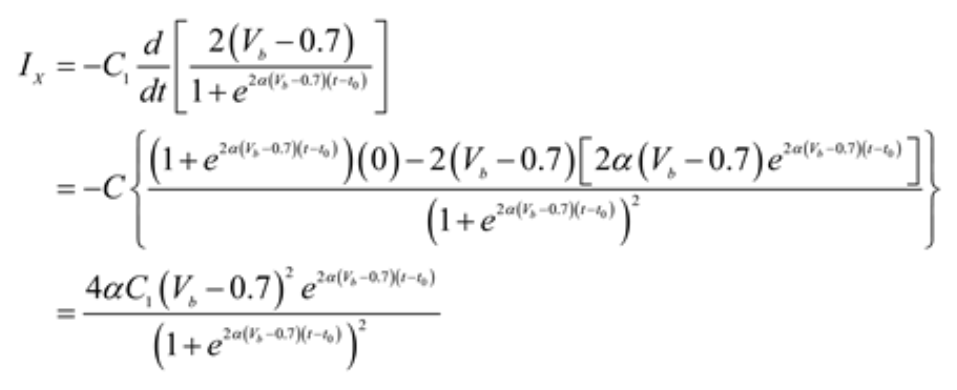
\includegraphics{2.9-2}
	\end{minipage}
\end{figure}


		\begin{figure}[H] %H为当前位置,!htb为忽略美学标准,htbp为浮动图形
	\begin{minipage}{\linewidth}
		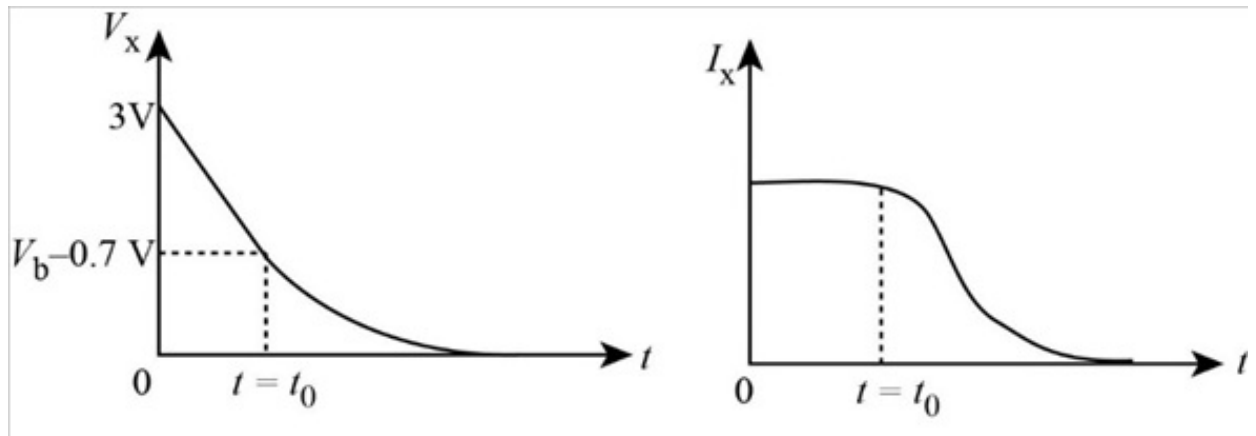
\includegraphics{2.9-1}
	\end{minipage}
	\caption*{图1} %最终文档中希望显示的图片标题
\end{figure}

\color{blue}{
	
	\{
	
	联立之后可得
	
			\begin{figure}[H] %H为当前位置,!htb为忽略美学标准,htbp为浮动图形
		\begin{minipage}{\linewidth}
			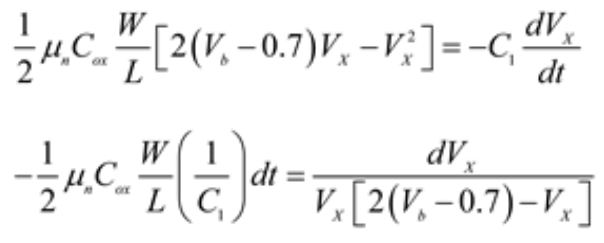
\includegraphics{2.9-3}
		\end{minipage}
	\end{figure}
	
	令$\alpha=\frac{1}{2}\mu_nC_{ox}\frac{W}{L}(\frac{1}{C_1})$
	
			\begin{figure}[H] %H为当前位置,!htb为忽略美学标准,htbp为浮动图形
		\begin{minipage}{\linewidth}
			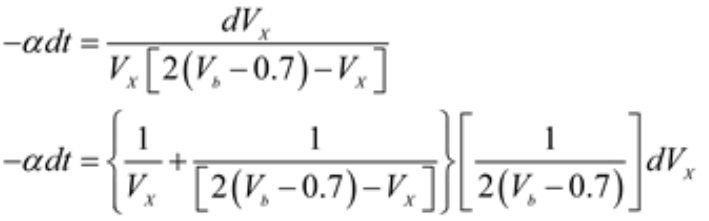
\includegraphics{2.9-4}
		\end{minipage}
	\end{figure}
	
			\begin{figure}[H] %H为当前位置,!htb为忽略美学标准,htbp为浮动图形
		\begin{minipage}{\linewidth}
			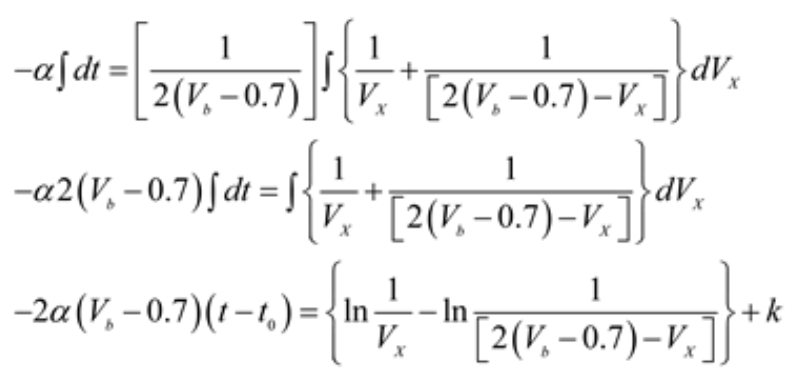
\includegraphics{2.9-5}
		\end{minipage}
	\end{figure}
	
	$2 \alpha (V_b-0.7)(t-t_0)=\{ln\frac{[2(V_b-0.7)-V_X]}{V_X}\}+k$\ding{172}
	
	把临界条件$t=t_0$和$V_X=V_b-0.7$代入上式
	
	
			\begin{figure}[H] %H为当前位置,!htb为忽略美学标准,htbp为浮动图形
		\begin{minipage}{\linewidth}
			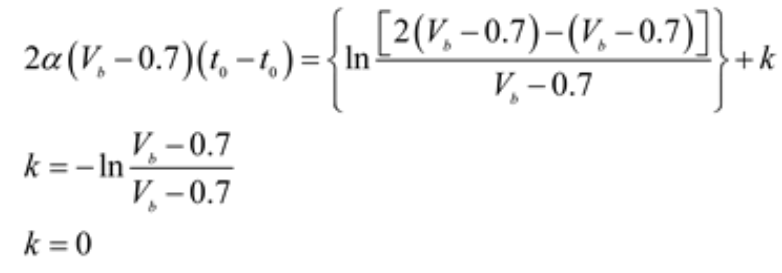
\includegraphics{2.9-6}
		\end{minipage}
	\end{figure}
	
	把$k=0$代入\ding{172}
	
			\begin{figure}[H] %H为当前位置,!htb为忽略美学标准,htbp为浮动图形
		\begin{minipage}{\linewidth}
			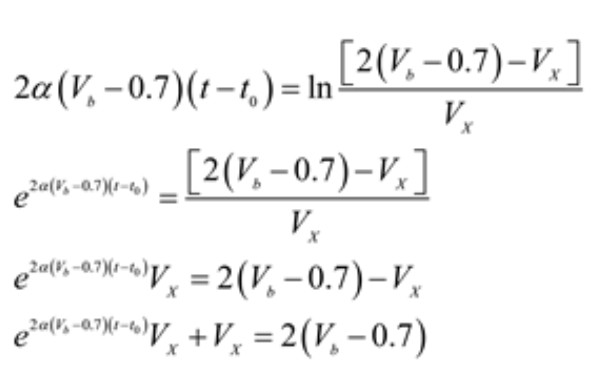
\includegraphics{2.9-7}
		\end{minipage}
	\end{figure}
	
			\begin{figure}[H] %H为当前位置,!htb为忽略美学标准,htbp为浮动图形
		\begin{minipage}{\linewidth}
			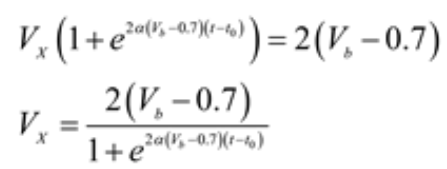
\includegraphics{2.9-8}
		\end{minipage}
	\end{figure}
	
	把上式代入$I_X=-C_1\frac{dV_X}{dt}$
	
			\begin{figure}[H] %H为当前位置,!htb为忽略美学标准,htbp为浮动图形
		\begin{minipage}{\linewidth}
			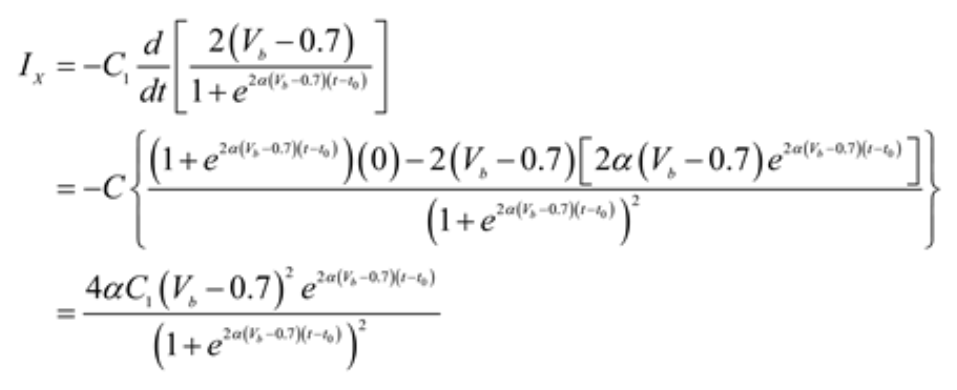
\includegraphics{2.9-2}
		\end{minipage}
	\end{figure}
	
	
	
	\}
	
}


\color{black}{
	
}


\scalebox{3}{(b)}

当$3V>V_{X}>0.7V$时,NFET在饱和区

$I_X=\frac{1}{2}\mu_nC_{ox}\frac{W}{L}(V_{X}-V_{TH})^2$

$-C_1\frac{dV_X}{dt}=\frac{1}{2}\mu_nC_{ox}\frac{W}{L}(V_{X}-0.7V)^2$

由上式最终可得$I_X=\frac{\alpha C_1}{(\alpha t+\frac{1}{2.3})^2}$



		\begin{figure}[H] %H为当前位置,!htb为忽略美学标准,htbp为浮动图形
	\begin{minipage}{\linewidth}
		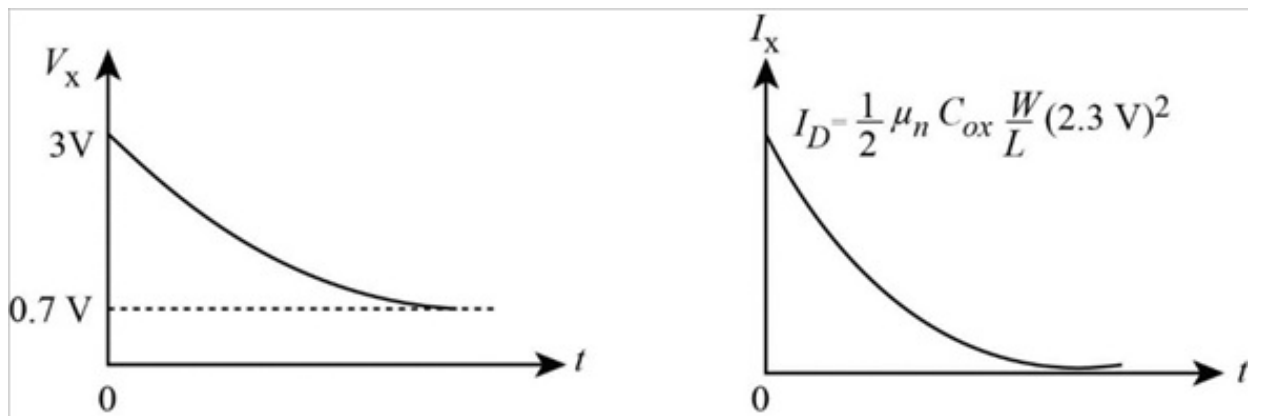
\includegraphics{2.9-9}
	\end{minipage}
	\caption*{图2} %最终文档中希望显示的图片标题
\end{figure}

\color{blue}{
	
	\{
	
	$-C_1\frac{dV_X}{dt}=\frac{1}{2}\mu_nC_{ox}\frac{W}{L}(V_{X}-0.7V)^2$
	
	$\frac{1}{2}\mu_nC_{ox}\frac{W}{L}(\frac{1}{C_1})dt=-\frac{dV_X}{(V_X-0.7V)^2}$
	
		$\alpha dt=-\frac{dV_X}{(V_X-0.7V)^2}$
		
			$\alpha \int dt=- \int \frac{dV_X}{(V_X-0.7V)^2}$
			
			$\alpha t=\frac{1}{V_X-0.7V}+k$
			
			$\alpha (0)=\frac{1}{(3)-0.7V}+k$
			
			$k=-\frac{1}{2.3}$
	
	把$k=-\frac{1}{2.3}$代入$\alpha t=\frac{1}{V_X-0.7V}+k$
	
	$\alpha t=\frac{1}{V_X-0.7V}-\frac{1}{2.3}$
	
	$\alpha t+\frac{1}{2.3}=\frac{1}{V_X-0.7V}$
	
	$V_X-0.7=\frac{1}{\alpha t+\frac{1}{2.3}}$
	
	$V_X=\frac{1}{\alpha t+\frac{1}{2.3}}+0.7$
	
	把上式代入$I_X=-C_1\frac{dV_X}{dt}$
	
	\begin{figure}[H] %H为当前位置,!htb为忽略美学标准,htbp为浮动图形
		\begin{minipage}{\linewidth}
			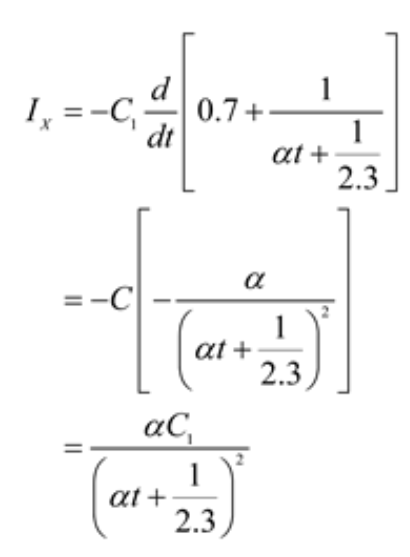
\includegraphics{2.9-10}
		\end{minipage}
	\end{figure}
	
	
	
	\}
	
}


\color{black}{
	
}


\scalebox{3}{(c)}

因为$V_{DS}=0$,因此NFET关

		\begin{figure}[H] %H为当前位置,!htb为忽略美学标准,htbp为浮动图形
	\begin{minipage}{\linewidth}
		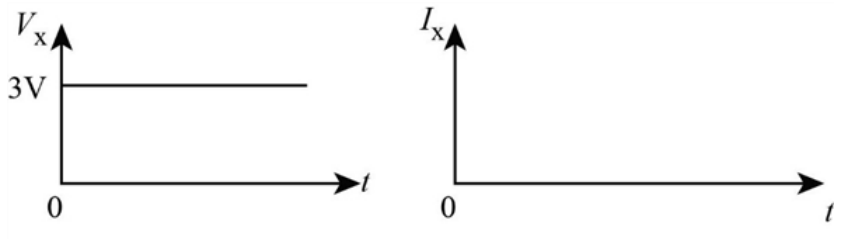
\includegraphics{2.9-11}
	\end{minipage}
	\caption*{图3} %最终文档中希望显示的图片标题
\end{figure}

\color{blue}{
	
	\{
	
因为$V_{DS}=0$,因此$V_{GS}-V_{TH}>V_{DS}=0$,使用线性区公式
	
	$I_X=\mu_nC_{ox}\frac{W}{L}[(V_{GS}-V_{TH})V_{DS}-\frac{1}{2}V_{DS}^2]=0$
	
	\}
	
}


\color{black}{
	
}

\scalebox{3}{(d)}

$I_X=-C_1\frac{dV_X}{dt}$

$I_1=-C_1\frac{dV_X}{dt}$

$\frac{dV_X}{dt}=-\frac{I_1}{C_1}$

$dV_X=-\frac{I_1}{C_1}dt$

$\int dV_X=-\frac{I_1}{C_1} \int dt$

$V_X=-\frac{I_1}{C_1}t+k$\ding{173}

代入初值

$3=-\frac{I_1}{C_1}(0)+k$

$k=3$

将上式代入\ding{173}

$V_X=-\frac{I_1}{C_1}t+3$

		\begin{figure}[H] %H为当前位置,!htb为忽略美学标准,htbp为浮动图形
	\begin{minipage}{\linewidth}
		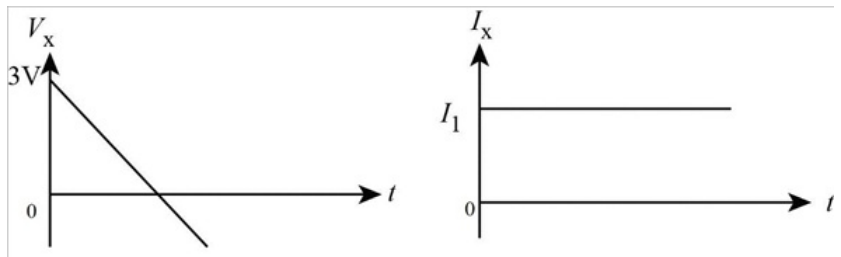
\includegraphics{2.9-12}
	\end{minipage}
	\caption*{图4} %最终文档中希望显示的图片标题
\end{figure}

\scalebox{3}{(e)}

		\begin{figure}[H] %H为当前位置,!htb为忽略美学标准,htbp为浮动图形
	\begin{minipage}{\linewidth}
		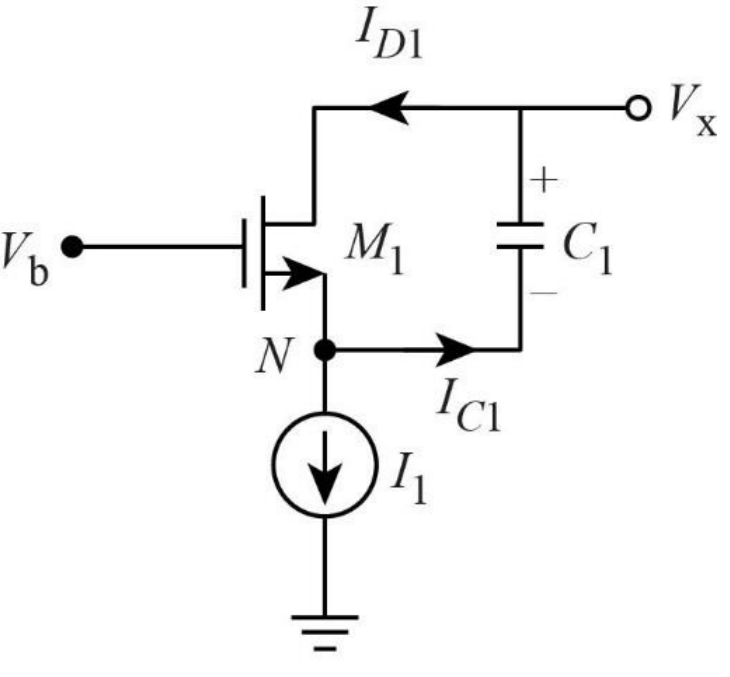
\includegraphics{2.9-13}
	\end{minipage}
	\caption*{图5} %最终文档中希望显示的图片标题
\end{figure}

当$t=0^+$时,NFET漏电流来自电容,$I_X=I_{C1}+I_1>I_1$。如果电流源是理想的,则N点电压跳至$-\infty$。如果$I_1$是不理想的,则n点电压跳至0并且电容通过NFET放电。





		\begin{figure}[H] %H为当前位置,!htb为忽略美学标准,htbp为浮动图形
	\begin{minipage}{\linewidth}
		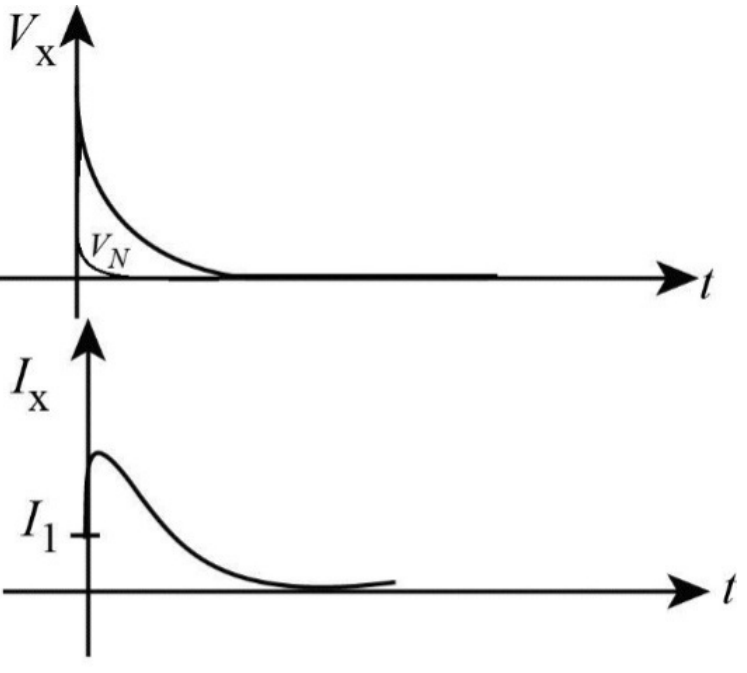
\includegraphics{2.9-14}
	\end{minipage}
	\caption*{图6} %最终文档中希望显示的图片标题
\end{figure}

\color{blue}{
	
	\{
	
	当$t=0^+$时,电子按电流反方向从地跑到N点和电容器上方降低电势,$V_N=0$后电子仅仅跑到电容器上方降低电势,$I_X=I_{D}$随着$V_{DS}=V_X-V_N$的减小而减小,由于$I_1$不理想因此最终$I_1=0$并且$I_1$两端电压为0
	
	
	
	\}
	
}


\color{black}{
	
}